\documentclass{article}%
\usepackage[T1]{fontenc}%
\usepackage[utf8]{inputenc}%
\usepackage{lmodern}%
\usepackage{textcomp}%
\usepackage{lastpage}%
\usepackage{parskip}%
\usepackage[top=5cm,hmargin=2cm,headheight=100pt,footskip=100pt,bottom=5cm]{geometry}%
\usepackage{amsmath}%
\usepackage{graphicx}%
\usepackage{needspace}%
\usepackage{color}%
\usepackage{longtable}%
\usepackage{multirow}%
\usepackage{tabularx}%
\usepackage[table]{xcolor}%
\usepackage{xcolor}%
\usepackage{fancyhdr}%
%
\definecolor{OsdagGreen}{RGB}{153,169,36}%
\definecolor{PassColor}{RGB}{153,169,36}%
\definecolor{Red}{RGB}{255,0,0}%
\definecolor{Green}{RGB}{0,200,0}%
\definecolor{FailColor}{HTML}{933A16}%
\fancypagestyle{header}{ 
\renewcommand{\headrulewidth}{0pt}%
\renewcommand{\footrulewidth}{0pt}%
\fancyhead{ 
}%
\fancyfoot{ 
}%
\fancyhead[C]{ 
\begin{tabularx}{\textwidth}{|l|p{4cm}|l|X|}%
\hline%
\multicolumn{2}{|c|}{}&\multicolumn{2}{|c|}{Created with%

\includegraphics[width=4.0cm,height=1cm]{/home/aaranyak/School_Work_Grade_9/Internship/Osdag_Dev/Osdag/ResourceFiles/images/Osdag_header_report.png}}\\%
\hline%
\rowcolor{OsdagGreen}%
Company Name&Daredevil Developers&Project Title&Osdag on Web\\%
\hline%
\rowcolor{OsdagGreen}%
Group/Team Name&Web Development Teams&Subtitle&\\%
\hline%
\rowcolor{OsdagGreen}%
Designer&Gyrnaskha Aahoa&Job Number&0\\%
\hline%
\rowcolor{OsdagGreen}%
Date&10 /03 /2023&Client&The No Name Guy\\%
\hline%
\end{tabularx}
}%
\fancyfoot[R]{ 
Page \thepage
}
}%
%
\begin{document}%
\normalsize%
\fontsize{8}{12}%
\selectfont%
\pagestyle{header}%
\section{Input Parameters}%
\label{sec:InputParameters}%
\renewcommand{\arraystretch}{1.2}%
\begin{longtable}{|p{5cm}|p{2.5cm}|p{1.5cm}|p{3cm}|p{3.5cm}|}%
\hline%
\hline%
\multicolumn{3}{|c|}{Main Module}&\multicolumn{2}{|c|}{Shear Connection}\\%
\hline%
\hline%
\multicolumn{3}{|c|}{Module}&\multicolumn{2}{|c|}{Fin Plate Connection}\\%
\hline%
\hline%
\multicolumn{3}{|c|}{Connectivity}&\multicolumn{2}{|c|}{Column Flange{-}Beam Web}\\%
\hline%
\hline%
\multicolumn{3}{|c|}{Shear Force (kN)}&\multicolumn{2}{|c|}{10.0}\\%
\hline%
\hline%
\multicolumn{3}{|c|}{Axial Force (kN)}&\multicolumn{2}{|c|}{30.0}\\%
\hline%
\hline%
\multicolumn{5}{|c|}{\textbf{Supporting Section {-} Mechanical Properties}}\\%
\hline%
\hline%
\multirow{13}{*}{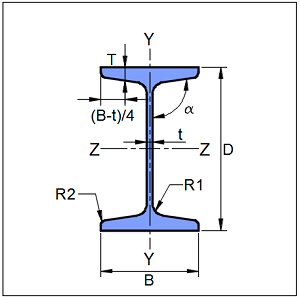
\includegraphics[width=5cm,height=5cm]{/home/aaranyak/School_Work_Grade_9/Internship/Osdag_Dev/Osdag/ResourceFiles/images/Slope_Beam.png}}&\multicolumn{2}{|c|}{Supporting Section}&\multicolumn{2}{|c|}{HB 150}\\%
\cline{2%
-%
5}%
&\multicolumn{2}{|c|}{Material}&\multicolumn{2}{|c|}{E 250 (Fe 410 W)A}\\%
\cline{2%
-%
5}%
&\multicolumn{2}{|c|}{Ultimate Strength, $F_u$ (MPa)}&\multicolumn{2}{|c|}{410}\\%
\cline{2%
-%
5}%
&\multicolumn{2}{|c|}{Yield Strength, $F_y$ (MPa)}&\multicolumn{2}{|c|}{250}\\%
\cline{2%
-%
5}%
&Mass, $m$ (kg/m)&27.06&$I_z$ (cm$^4$)&1450.0\\%
\cline{2%
-%
5}%
&Area, $A$ (cm$^2$)&34.4&$I_y$(cm$^4$)&431.0\\%
\cline{2%
-%
5}%
&$D$ (mm)&150.0&$r_z$ (cm)&6.49\\%
\cline{2%
-%
5}%
&$B$ (mm)&150.0&$r_y$ (cm)&3.53\\%
\cline{2%
-%
5}%
&$t$ (mm)&5.4&$Z_z$ (cm$^3$)&194.0\\%
\cline{2%
-%
5}%
&$T$ (mm)&9&$Z_y$ (cm$^3$)&57.5\\%
\cline{2%
-%
5}%
&Flange Slope&94&$Z_{pz}$ (cm$^3$)&215.0\\%
\cline{2%
-%
5}%
&$R_1$ (mm)&8.0&$Z_{py}$ (cm$^3$)&92.7\\%
\cline{2%
-%
5}%
&$R_2$ (mm)&4.0&&\\%
\cline{2%
-%
5}%
\hline%
\multicolumn{5}{|c|}{\textbf{Supported Section {-} Mechanical Properties}}\\%
\hline%
\hline%
\multirow{13}{*}{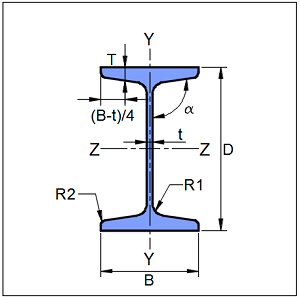
\includegraphics[width=5cm,height=5cm]{/home/aaranyak/School_Work_Grade_9/Internship/Osdag_Dev/Osdag/ResourceFiles/images/Slope_Beam.png}}&\multicolumn{2}{|c|}{Supported Section}&\multicolumn{2}{|c|}{JB 150}\\%
\cline{2%
-%
5}%
&\multicolumn{2}{|c|}{Material}&\multicolumn{2}{|c|}{E 250 (Fe 410 W)A}\\%
\cline{2%
-%
5}%
&\multicolumn{2}{|c|}{Ultimate Strength, $F_u$ (MPa)}&\multicolumn{2}{|c|}{410}\\%
\cline{2%
-%
5}%
&\multicolumn{2}{|c|}{Yield Strength, $F_y$ (MPa)}&\multicolumn{2}{|c|}{250}\\%
\cline{2%
-%
5}%
&Mass, $m$ (kg/m)&7.07&$I_z$ (cm$^4$)&321.0\\%
\cline{2%
-%
5}%
&Area, $A$ (cm$^2$)&9.0&$I_y$(cm$^4$)&9.21\\%
\cline{2%
-%
5}%
&$D$ (mm)&150.0&$r_z$ (cm)&5.97\\%
\cline{2%
-%
5}%
&$B$ (mm)&50.0&$r_y$ (cm)&1.01\\%
\cline{2%
-%
5}%
&$t$ (mm)&3.0&$Z_z$ (cm$^3$)&42.8\\%
\cline{2%
-%
5}%
&$T$ (mm)&4.6&$Z_y$ (cm$^3$)&3.68\\%
\cline{2%
-%
5}%
&Flange Slope&91.5&$Z_{pz}$ (cm$^3$)&49.5\\%
\cline{2%
-%
5}%
&$R_1$ (mm)&5.0&$Z_{py}$ (cm$^3$)&5.96\\%
\cline{2%
-%
5}%
&$R_2$ (mm)&1.5&&\\%
\cline{2%
-%
5}%
\hline%
\multicolumn{5}{|c|}{\textbf{Bolt Details {-} Input and Design Preference}}\\%
\hline%
\multicolumn{3}{|c|}{\multirow{2}{*}{Diameter (mm)}}&\multicolumn{2}{|c|}{{[}8, 10, 12, 14, 16, 18, 20, 22, 24, 27, 30, 33, 36, 39, }\\%
\multicolumn{3}{|c|}{\multirow{2}{*}{}}&\multicolumn{2}{|c|}{42, 45, 48, 52, 56, 60, 64{]}}\\%
\hline%
\multicolumn{3}{|c|}{\multirow{2}{*}{Property Class}}&\multicolumn{2}{|c|}{{[}'3.6', '4.6', '4.8', '5.6', '5.8', '6.8', '8.8', '9.8',}\\%
\multicolumn{3}{|c|}{\multirow{2}{*}{}}&\multicolumn{2}{|c|}{ '10.9', '12.9'{]}}\\%
\hline%
\hline%
\multicolumn{3}{|c|}{Type}&\multicolumn{2}{|c|}{Bearing Bolt}\\%
\hline%
\hline%
\multicolumn{3}{|c|}{Hole Type}&\multicolumn{2}{|c|}{Standard}\\%
\hline%
\hline%
\multicolumn{3}{|c|}{Bolt Tension}&\multicolumn{2}{|c|}{Non pre{-}tensioned}\\%
\hline%
\hline%
\multicolumn{3}{|c|}{Slip Factor, ($\mu_{f}$)}&\multicolumn{2}{|c|}{0.3}\\%
\hline%
\hline%
\multicolumn{5}{|c|}{\textbf{Detailing {-} Design Preference}}\\%
\hline%
\hline%
\multicolumn{3}{|c|}{Edge Preparation Method}&\multicolumn{2}{|c|}{Sheared or hand flame cut}\\%
\hline%
\hline%
\multicolumn{3}{|c|}{Gap Between Members (mm)}&\multicolumn{2}{|c|}{10.0}\\%
\hline%
\hline%
\multicolumn{3}{|c|}{Are the Members Exposed to Corrosive Influences?}&\multicolumn{2}{|c|}{False}\\%
\hline%
\hline%
\multicolumn{5}{|c|}{\textbf{Plate Details {-} Input and Design Preference}}\\%
\hline%
\multicolumn{3}{|c|}{\multirow{2}{*}{Thickness (mm)}}&\multicolumn{2}{|c|}{{[}8, 10, 12, 14, 16, 18, 20, 22, 25, 28, 32, 36, 40, 45, }\\%
\multicolumn{3}{|c|}{\multirow{2}{*}{}}&\multicolumn{2}{|c|}{50, 56, 63, 75, 80, 90, 100, 110, 120{]}}\\%
\hline%
\hline%
\multicolumn{3}{|c|}{Material}&\multicolumn{2}{|c|}{E 250 (Fe 410 W)A}\\%
\hline%
\hline%
\multicolumn{3}{|c|}{Ultimate Strength, Fu (MPa)}&\multicolumn{2}{|c|}{410}\\%
\hline%
\hline%
\multicolumn{3}{|c|}{Yield Strength, Fy (MPa)}&\multicolumn{2}{|c|}{250}\\%
\hline%
\hline%
\multicolumn{5}{|c|}{\textbf{Weld Details {-} Input and Design Preference}}\\%
\hline%
\hline%
\multicolumn{3}{|c|}{Weld Type}&\multicolumn{2}{|c|}{Fillet}\\%
\hline%
\hline%
\multicolumn{3}{|c|}{Type of Weld Fabrication}&\multicolumn{2}{|c|}{Shop Weld}\\%
\hline%
\hline%
\multicolumn{3}{|c|}{Material Grade Overwrite, Fu (MPa)}&\multicolumn{2}{|c|}{410.0}\\%
\hline%
\end{longtable}

%
\Needspace{10\baselineskip}%
\newpage%
\section{Design Checks}%
\label{sec:DesignChecks}%
\renewcommand{\arraystretch}{1.2}%
\begin{tabularx}{\textwidth}{|>{\centering}p{12.5cm}|>{\centering\arraybackslash}X|}%
\hline%
\textbf{Design Status}&\cellcolor{Red}{\textbf{Fail}}\\%
\hline%
\end{tabularx}%
\subsection{Initial Section Check}%
\label{subsec:InitialSectionCheck}%
\renewcommand{\arraystretch}{1.2}%
\begin{longtable}{|p{4cm}|p{5cm}|p{5.5cm}|p{1.5cm}|}%
\hline%
\rowcolor{OsdagGreen}%
Check&Required&Provided&Remarks\\%
\hline%
\endhead%
\hline%
Shear Yielding Capacity (kN)&10.0&$\begin{aligned} V_{d_y} &= \frac{A_vf_y}{\sqrt{3}\gamma_{m0}}\\ &=\frac{150.0\times3.0\times250}{\sqrt{3} \times1.1 \times 1000}\\ &=59.05 \\ \\ & [\text{Ref. IS ~800:2007,~Cl.10.4.3}] \end{aligned}$&\textcolor{OsdagGreen}{ 
\textbf{Pass}
}\\%
\hline%
Allowable Shear Capacity (kN)&10.0&$\begin{aligned} V_{d} &= 0.6~V_{dy}\\ &=0.6 \times59.05\\ &=35.43\\ \\ & [\text{Limited to low shear}] \end{aligned}$&\textcolor{OsdagGreen}{ 
\textbf{Pass}
}\\%
\hline%
Tension Yielding Capacity (kN)&30.0&$\begin{aligned} T_{\text{dg}} &= \frac{A_g f_y}{\gamma_{m0}}\\ \\ A_{g} &= l t =150.0\times3.0\\ &=\frac{450.0\times250}{1.1\times 10^3}\\ &=102.27\\ \\ & [\text{Ref. IS 800:2007, Cl.6.2}] \end{aligned}$&\textcolor{OsdagGreen}{ 
\textbf{Pass}
}\\%
\hline%
\end{longtable}

%
\Needspace{10\baselineskip}%
\subsection{Load Consideration}%
\label{subsec:LoadConsideration}%
\renewcommand{\arraystretch}{1.2}%
\begin{longtable}{|p{4cm}|p{5cm}|p{5.5cm}|p{1.5cm}|}%
\hline%
\rowcolor{OsdagGreen}%
Check&Required&Provided&Remarks\\%
\hline%
\endhead%
\hline%
Applied Axial Force (kN)&30.0&30.0&\textcolor{OsdagGreen}{ 
\textbf{}
}\\%
\hline%
Applied Shear Force (kN)&10.0&$\begin{aligned} {V_{y}}_{\text{min}} &=  \min(0.15 V_{d_y},~ 40.0)\\ & =  \min(0.15 \times59.05,~ 40.0)\\ &=40\\ \\  V_u~~ &= \max(V_{y},~ {V_{y}}_{\text{min}})\\ &=  \max(10.0,40)\\ &=40\\ \\ & [ \text{Ref. IS 800:2007, Cl.10.7}] \end{aligned}$&\textcolor{OsdagGreen}{ 
\textbf{}
}\\%
\hline%
\end{longtable}

%
\Needspace{10\baselineskip}%
\subsection{Bolt Design}%
\label{subsec:BoltDesign}%
\renewcommand{\arraystretch}{1.2}%
\begin{longtable}{|p{3.5cm}|p{5.3cm}|p{6.7cm}|p{1.5cm}|}%
\hline%
\rowcolor{OsdagGreen}%
Check&Required&Provided&Remarks\\%
\hline%
\endhead%
\hline%
Diameter (mm)&&10.0&\textcolor{OsdagGreen}{ 
\textbf{}
}\\%
\hline%
Property Class&&6.8&\textcolor{OsdagGreen}{ 
\textbf{}
}\\%
\hline%
Plate Thickness (mm)&$\begin{aligned} t_w=3.0\end{aligned}$&8.0&\textcolor{OsdagGreen}{ 
\textbf{Pass}
}\\%
\hline%
No. of Bolt Columns&&1&\textcolor{OsdagGreen}{ 
\textbf{Pass}
}\\%
\hline%
No. of Bolt Rows&&3&\textcolor{OsdagGreen}{ 
\textbf{}
}\\%
\hline%
Min. Pitch Distance (mm)&$\begin{aligned}p_{\min}&= 2.5 d\\ &=2.5 \times10.0\\&=25.0\\ \\ & [\text{Ref. IS 800:2007, Cl.10.2.2}] \end{aligned}$&40&\textcolor{OsdagGreen}{ 
\textbf{Pass}
}\\%
\hline%
Max. Pitch Distance (mm)&$\begin{aligned}p/g_{\max}&=\min(32t,~300)\\ &=\min(32\times3.0,~ 300) \\ &=\min(96.0,~ 300) \\ &=96.0 \\ \\ \text{Where},~t &= \min(8.0,3.0)\\ \\ & [\text{Ref. IS 800:2007, Cl.10.2.3}] \end{aligned}$&40&\textcolor{OsdagGreen}{ 
\textbf{Pass}
}\\%
\hline%
Min. Gauge Distance (mm)&$\begin{aligned}p_{\min}&= 2.5 d\\ &=2.5 \times10.0\\&=25.0\\ \\ & [\text{Ref. IS 800:2007, Cl.10.2.2}] \end{aligned}$&0.0&\textcolor{OsdagGreen}{ 
\textbf{}
}\\%
\hline%
Max. Gauge Distance (mm)&$\begin{aligned}p/g_{\max}&=\min(32t,~300)\\ &=\min(32\times3.0,~ 300) \\ &=\min(96.0,~ 300) \\ &=96.0 \\ \\ \text{Where},~t &= \min(8.0,3.0)\\ \\ & [\text{Ref. IS 800:2007, Cl.10.2.3}] \end{aligned}$&0.0&\textcolor{OsdagGreen}{ 
\textbf{}
}\\%
\hline%
Min. End Distance (mm)&$\begin{aligned}e_{\min} &= 1.7 d_0 \\ &= 1.7\times10\\ &=17.0\\ \\ & [\text{Ref. IS 800:2007, Cl.10.2.4.2}] \end{aligned}$&20&\textcolor{OsdagGreen}{ 
\textbf{Pass}
}\\%
\hline%
Max. End Distance (mm)&$\begin{aligned}e_{\max} &= 12 t \varepsilon ;~\varepsilon = \sqrt{\frac{250}{f_y}}\\ e_1 &= 12 \times 8.0\times \sqrt{\frac{250}{250}} = 96.0\\ e_2 &= 12 \times3.0\times\sqrt{\frac{250}{250}} = 36.0\\ e_{\max}&=\min(e_1,~e_2)=36.0 \\ \\ & [\text{Ref. IS 800:2007, Cl.10.2.4.3}] \end{aligned}$&20&\textcolor{OsdagGreen}{ 
\textbf{Pass}
}\\%
\hline%
Min. Edge Distance (mm)&$\begin{aligned}e\textquotesingle_{\min} &= 1.7 d_0 \\ &= 1.7\times10\\ &=17.0\\ \\ & [\text{Ref. IS 800:2007, Cl.10.2.4.2}] \end{aligned}$&20&\textcolor{OsdagGreen}{ 
\textbf{Pass}
}\\%
\hline%
Max. Edge Distance (mm)&$\begin{aligned}e\textquotesingle_{\max} &= 12 t \varepsilon ;~\varepsilon = \sqrt{\frac{250}{f_y}}\\ e_1 &= 12 \times 8.0\times \sqrt{\frac{250}{250}} = 96.0\\ e_2 &= 12 \times3.0\times\sqrt{\frac{250}{250}} = 36.0\\ e\textquotesingle_{\max}&=min(e_1,~e_2)=36.0 \\ \\ & [\text{Ref. IS 800:2007, Cl.10.2.4.3}] \end{aligned}$&20&\textcolor{OsdagGreen}{ 
\textbf{Pass}
}\\%
\hline%
Moment Demand (kNm)&&$\begin{aligned}  M_d &= (V_u \times \text{ecc} + M_w)\\ \\ & \text{ecc = eccentricity} \\ & M_w = \text{external moment acting on web} \\ \\  &= \frac{(10.0 \times 10^3 \times30.0 + 0.0\times10^6)}{10^6}\\  & =0.3\end{aligned}$&\textcolor{OsdagGreen}{ 
\textbf{}
}\\%
\hline%
Bolt Force Parameter(s) (mm)&$\begin{aligned} l_n~~~ &= \text{length available} \\  l_n~~~ &= p~(n_r - 1)\\  &= 40 \times (3 - 1)\\  & =80\\ \\  y_{\text{max}} &= l_n / 2\\  &= 80 / 2 \\  & =40.0\\ \\ x_{\text{max}} &= g(n_c - 1)/2 \\  &= 0.0 \times (1 - 1) / 2 \\  & =0.0\end{aligned}$&&\textcolor{OsdagGreen}{ 
\textbf{}
}\\%
\hline%
Bolt Force (kN)&$\begin{aligned} vbv~~ &= V_u / (n_r \times n_c)\\  &= \frac{10.0}{ (3\times1)}\\  & =3.33\\ \\ tmh~ &= \frac{M_d \times y_{\text{max}} }{ \Sigma r_i^2} \\  &= \frac{0.3\times40.0}{3.2}\\  & =3.75\\ \\  tmv ~&= \frac{M_d \times x_{\text{max}}}{\Sigma r_i^2}\\ &= \frac{0.3\times 0.0}{3.2}\\  & =0.0\\ \\  abh~ & = \frac{A_u }{(n_r \times n_c)}\\   & =\frac{30.0}{ (3 \times1)}\\  & =10.0\\ \\  v_{\text{res}} &=\sqrt{(vbv +tmv) ^ 2 + (tmh+abh) ^ 2}\\   &= \sqrt{(3.33 +0.0) ^2 + (3.75+10.0) ^ 2}\\  & =14.15\end{aligned}$&&\textcolor{OsdagGreen}{ 
\textbf{}
}\\%
\hline%
Shear Capacity (kN)&&$\begin{aligned}V_{\text{dsb}} &= \frac{f_{ub} n_n A_{nb}}{\sqrt{3} \gamma_{mb}}\\ &= \frac{600.0\times1\times58}{1000\times\sqrt{3}~\times~1.25}\\ &= 16.07\\ \\ & [\text{Ref. IS 800:2007, Cl.10.3.3}] \end{aligned}$&\textcolor{OsdagGreen}{ 
\textbf{}
}\\%
\hline%
Kb& &$\begin{aligned} k_b & = \min \Bigg(\frac{e}{3d_0},~\frac{p}{3d_0}-0.25,~\frac{f_{ub}}{f_u},~1.0 \Bigg) \\ & = \min \Bigg(\frac{20}{3\times10},~\frac{40}{3\times10}-0.25,~\frac{600.0}{410},~1.0 \Bigg)\\ & = \min(0.67,1.08,1.46,1.0)\\ & = 0.67\\ \\ & [\text{Ref. IS 800:2007, Cl.10.3.4}] \end{aligned}$&\textcolor{OsdagGreen}{ 
\textbf{}
}\\%
\hline%
Bearing Capacity (kN)&&$\begin{aligned}V_{\text{dpb}} &= \frac{2.5 k_b d t f_u}{\gamma_{mb}}\\ &= \frac{2.5 \times 0.67\times10.0\times3.0\times410}{1000\times1.25}\\ &=16.48\\ \\ & [\text{Ref. IS 800:2007, Cl.10.3.4}] \end{aligned}$&\textcolor{OsdagGreen}{ 
\textbf{}
}\\%
\hline%
Capacity (kN)&&$\begin{aligned} V_{\text{db}} &= \min~ (V_{\text{dsb}},~ V_{\text{dpb}})\\ &= \min~ (16.07,~16.48)\\ &=16.07\\ \\ & [\text{Ref. IS 800:2007, Cl.10.3.2}] \end{aligned}$&\textcolor{OsdagGreen}{ 
\textbf{}
}\\%
\hline%
Long Joint Reduction Factor&$\begin{aligned} & \text{if} ~l_j\geq 15 d~\text{then}~V_{\text{rd}} = \beta_{lj} V_{\text{db}} \\ \\ & \text{if}~l_j < 15 d~\text{then}~V_{\text{rd}} = V_{\text{db}} \\ \\ & \text{where},\\ & l_j = ((nc~\text{or}~nr) - 1) \times (p~\text{or}~g) \\ \\ & \beta_{lj} = 1.075 - l/(200 d) \\ & \text{but}~0.75\leq\beta_{lj}\leq1.0 \\ \\ & [\text{Ref. IS 800:2007, Cl.10.3.3.1}] \end{aligned}$&$\begin{aligned} l_j &= (n_r - 1) \times  p \\  &= (3 - 1) \times 40=80\\ \\  l&= 80\\  15 \times d &= 15 \times 10.0 = 150.0 \\ \\ & \text{since},~l_j < 15 \times d~\text{then}~\beta_{lj} = 1.0 \\ \\ &[ \text{Ref. IS 800:2007, Cl.10.3.3.1}] \end{aligned}$&\textcolor{OsdagGreen}{ 
\textbf{}
}\\%
\hline%
Capacity (kN)&14.15&16.07&\textcolor{OsdagGreen}{ 
\textbf{Pass}
}\\%
\hline%
\end{longtable}

%
\Needspace{10\baselineskip}%
\subsection{Plate Design}%
\label{subsec:PlateDesign}%
\renewcommand{\arraystretch}{1.2}%
\begin{longtable}{|p{3.5cm}|p{5cm}|p{6cm}|p{1.5cm}|}%
\hline%
\rowcolor{OsdagGreen}%
Check&Required&Provided&Remarks\\%
\hline%
\endhead%
\hline%
Min. Plate Height (mm)&$\begin{aligned} & 0.6 \times (d_b - 2 \times t_f - 2 \times r_r)\\ &= 0.6 \times (150.0- 2 \times4.6- 2 \times5.0)\\ &=78.48\\ \\ & [\text{Ref. INSDAG, Ch.5, sec.5.2.3}] \end{aligned}$&120&\textcolor{OsdagGreen}{ 
\textbf{Pass}
}\\%
\hline%
Max. Plate Height (mm)&$\begin{aligned} &d_b - 2 (t_{bf} + r_{b1} + \text{gap})\\ &=150.0- 2\times (4.6+5.0+ 10)\\ &=130.8\end{aligned}$&120&\textcolor{OsdagGreen}{ 
\textbf{Pass}
}\\%
\hline%
Min. Plate Width (mm)&$\begin{aligned} &2e_{\text{min}} + (n_c-1) p_{\text{min}})\\ &=2\times17.0+(1-1)  \times  25.0\\ &=44.0\end{aligned}$&50.0&\textcolor{OsdagGreen}{ 
\textbf{Pass}
}\\%
\hline%
Min. Plate Thickness (mm)&$\begin{aligned} t_w=3.0\end{aligned}$&8.0&\textcolor{OsdagGreen}{ 
\textbf{Pass}
}\\%
\hline%
Shear Yielding Capacity (kN)&&$\begin{aligned} V_{d_y} &= \frac{A_vf_y}{\sqrt{3}\gamma_{m0}}\\ &=\frac{120\times8.0\times250}{\sqrt{3} \times1.1 \times 1000}\\ &=125.97 \\ \\ & [\text{Ref. IS ~800:2007,~Cl.10.4.3}] \end{aligned}$&\textcolor{OsdagGreen}{ 
\textbf{}
}\\%
\hline%
Allowable Shear Capacity (kN)&$\begin{aligned} V &=10.0 \end{aligned}$&$\begin{aligned} V_{d} &= 0.6~V_{dy}\\ &=0.6 \times125.97\\ &=75.58\\ \\ & [\text{Limited to low shear}] \end{aligned}$&\textcolor{OsdagGreen}{ 
\textbf{Pass}
}\\%
\hline%
Shear Rupture Capacity (kN)&&$\begin{aligned} V_{d_n} &= \frac{0.75 A_{v_n} f_u}{\sqrt{3} \gamma_{m1}}\\ &=1\times \frac{(120-(3\times10))\times8.0\times410}{\sqrt{3}\times1.25}\\ &=221.4\\ \\ & [\text{ Ref. AISC, sect. J4}] \end{aligned}$&\textcolor{OsdagGreen}{ 
\textbf{}
}\\%
\hline%
Block Shear Capacity in Shear (kN)&&$\begin{aligned}V_{\text{dbl1}} &= \frac{A_{\text{vg}} f_{y}}{\sqrt{3} \gamma_{m0}} + \frac{0.9 A_{tn} f_{u}}{\gamma_{m1}}\\ \\ V_{\text{dbl2}} &= \frac{0.9A_{vn} f_{u}}{\sqrt{3} \gamma_{m1}} + \frac{A_{tg} f_{y}}{\gamma_{m0}}\\ \\ V_{\text{db}} &= \min(V_{db1},~ V_{db2})= 138.62\\ \\ & [\text{Ref. IS 800:2007, Cl.6.4}] \end{aligned}$&\textcolor{OsdagGreen}{ 
\textbf{}
}\\%
\hline%
Shear Capacity (kN)&10.0&$\begin{aligned} V_d &= \min(S_c,~V_{d_n},~V_{d_b})\\ &= \min(75.58,~221.4,~138.62)\\ &=75.58\\ \\ & [\text{ Ref. IS 800:2007, Cl.6.1}] \end{aligned}$&\textcolor{OsdagGreen}{ 
\textbf{Pass}
}\\%
\hline%
Tension Yielding Capacity (kN)&&$\begin{aligned} T_{\text{dg}} &= \frac{A_g f_y}{\gamma_{m0}}\\ \\ A_{g} &= l t =120\times8.0\\ &=\frac{960.0\times250}{1.1\times 10^3}\\ &=218.18\\ \\ & [\text{Ref. IS 800:2007, Cl.6.2}] \end{aligned}$&\textcolor{OsdagGreen}{ 
\textbf{}
}\\%
\hline%
Tension Rupture Capacity (kN)&&$\begin{aligned} T_{\text{dn}} &= \frac{0.9 A_{n} f_u}{\gamma_{m1}}\\ &=\frac{1\times~0.9\times (120-3\times10)\times8.0\times410}{1.25}\\ &=259.78\\ \\ & [\text{Ref. IS 800:2007, Cl.6.3.1}] \end{aligned}$&\textcolor{OsdagGreen}{ 
\textbf{}
}\\%
\hline%
Block Shear Capacity in Tension (kN)&&$\begin{aligned}T_{\text{dbl1}} &= \frac{A_{\text{vg}} f_{y}}{\sqrt{3} \gamma_{m0}} + \frac{0.9 A_{tn} f_{u}}{\gamma_{m1}}\\ \\ T_{\text{dbl2}} &= \frac{0.9A_{vn} f_{u}}{\sqrt{3} \gamma_{m1}} + \frac{A_{tg} f_{y}}{\gamma_{m0}}\\ \\ T_{\text{db}} &= \min(T_{db1},~ T_{db2})= 183.69\\ \\ & [\text{Ref. IS 800:2007, Cl.6.4}] \end{aligned}$&\textcolor{OsdagGreen}{ 
\textbf{}
}\\%
\hline%
Tension Capacity (kN)&30.0&$\begin{aligned} T_{\text{d}} &= \min(T_{\text{dg}},~T_{\text{dn}},~T_{\text{db}})\\ &= \min(218.18,259.78,183.69)\\ &=183.69\\ \\ & [\text{Ref.IS 800:2007, Cl.6.1}] \end{aligned}$&\textcolor{OsdagGreen}{ 
\textbf{Pass}
}\\%
\hline%
Moment Capacity (kNm)&0.3&$\begin{aligned} {M_{d}}_{\text{z}} &= \frac{\beta_b Z_p fy}{\gamma_{m0} \times 10^6}\\ &=\frac{1.0\times28800.0\times250}{1.1 \times 10^6}\\ &=6.55\\ \\ & [\text{Ref. IS 800:2007, Cl.8.2.1.2}] \end{aligned}$&\textcolor{OsdagGreen}{ 
\textbf{Pass}
}\\%
\hline%
Interaction Ratio&$\begin{aligned} \leq1\end{aligned}$&$\begin{aligned} &\frac{0.3}{6.55}+\frac{30.0}{183.69}=0.21\\ \\ & [\text{Ref. IS 800:2007, Cl.10.7}] \end{aligned}$&\textcolor{OsdagGreen}{ 
\textbf{Pass}
}\\%
\hline%
\end{longtable}

%
\Needspace{10\baselineskip}%
\subsection{Section Design}%
\label{subsec:SectionDesign}%
\renewcommand{\arraystretch}{1.2}%
\begin{longtable}{|p{3.5cm}|p{5cm}|p{6cm}|p{1.5cm}|}%
\hline%
\rowcolor{OsdagGreen}%
Check&Required&Provided&Remarks\\%
\hline%
\endhead%
\hline%
Shear Yielding Capacity (kN)&&$\begin{aligned} V_{d_y} &= \frac{A_vf_y}{\sqrt{3}\gamma_{m0}}\\ &=\frac{150.0\times3.0\times250}{\sqrt{3} \times1.1 \times 1000}\\ &=59.05 \\ \\ & [\text{Ref. IS ~800:2007,~Cl.10.4.3}] \end{aligned}$&\textcolor{OsdagGreen}{ 
\textbf{}
}\\%
\hline%
Allowable Shear Capacity (kN)&$\begin{aligned} V &=10.0 \end{aligned}$&$\begin{aligned} V_{d} &= 0.6~V_{dy}\\ &=0.6 \times59.05\\ &=35.43\\ \\ & [\text{Limited to low shear}] \end{aligned}$&\textcolor{OsdagGreen}{ 
\textbf{Pass}
}\\%
\hline%
Shear Rupture Capacity (kN)&&$\begin{aligned} V_{d_n} &= \frac{0.75 A_{v_n} f_u}{\sqrt{3} \gamma_{m1}}\\ &=1\times \frac{(150.0-(3\times10))\times3.0\times410}{\sqrt{3}\times1.25}\\ &=110.7\\ \\ & [\text{ Ref. AISC, sect. J4}] \end{aligned}$&\textcolor{OsdagGreen}{ 
\textbf{}
}\\%
\hline%
Block Shear Capacity in Shear (kN)&&$\begin{aligned}V_{\text{dbl1}} &= \frac{A_{\text{vg}} f_{y}}{\sqrt{3} \gamma_{m0}} + \frac{0.9 A_{tn} f_{u}}{\gamma_{m1}}\\ \\ V_{\text{dbl2}} &= \frac{0.9A_{vn} f_{u}}{\sqrt{3} \gamma_{m1}} + \frac{A_{tg} f_{y}}{\gamma_{m0}}\\ \\ V_{\text{db}} &= \min(V_{db1},~ V_{db2})= 51.98\\ \\ & [\text{Ref. IS 800:2007, Cl.6.4}] \end{aligned}$&\textcolor{OsdagGreen}{ 
\textbf{}
}\\%
\hline%
Shear Capacity (kN)&10.0&$\begin{aligned} V_d &= \min(S_c,~V_{d_n},~V_{d_b})\\ &= \min(35.43,~110.7,~51.98)\\ &=35.43\\ \\ & [\text{ Ref. IS 800:2007, Cl.6.1}] \end{aligned}$&\textcolor{OsdagGreen}{ 
\textbf{Pass}
}\\%
\hline%
Tension Yielding Capacity (kN)&&$\begin{aligned} T_{\text{dg}} &= \frac{A_g f_y}{\gamma_{m0}}\\ \\ A_{g} &= l t =150.0\times3.0\\ &=\frac{450.0\times250}{1.1\times 10^3}\\ &=102.27\\ \\ & [\text{Ref. IS 800:2007, Cl.6.2}] \end{aligned}$&\textcolor{OsdagGreen}{ 
\textbf{}
}\\%
\hline%
Tension Rupture Capacity (kN)&&$\begin{aligned} T_{\text{dn}} &= \frac{0.9 A_{n} f_u}{\gamma_{m1}}\\ &=\frac{1\times~0.9\times (150.0-3\times10)\times3.0\times410}{1.25}\\ &=106.27\\ \\ & [\text{Ref. IS 800:2007, Cl.6.3.1}] \end{aligned}$&\textcolor{OsdagGreen}{ 
\textbf{}
}\\%
\hline%
Block Shear Capacity in Tension (kN)&&$\begin{aligned}T_{\text{dbl1}} &= \frac{A_{\text{vg}} f_{y}}{\sqrt{3} \gamma_{m0}} + \frac{0.9 A_{tn} f_{u}}{\gamma_{m1}}\\ \\ T_{\text{dbl2}} &= \frac{0.9A_{vn} f_{u}}{\sqrt{3} \gamma_{m1}} + \frac{A_{tg} f_{y}}{\gamma_{m0}}\\ \\ T_{\text{db}} &= \min(T_{db1},~ T_{db2})= 68.88\\ \\ & [\text{Ref. IS 800:2007, Cl.6.4}] \end{aligned}$&\textcolor{OsdagGreen}{ 
\textbf{}
}\\%
\hline%
Tension Capacity (kN)&30.0&$\begin{aligned} T_{\text{d}} &= \min(T_{\text{dg}},~T_{\text{dn}},~T_{\text{db}})\\ &= \min(102.27,106.27,68.88)\\ &=68.88\\ \\ & [\text{Ref.IS 800:2007, Cl.6.1}] \end{aligned}$&\textcolor{OsdagGreen}{ 
\textbf{Pass}
}\\%
\hline%
Moment Capacity (kNm)&0.3&$\begin{aligned} {M_{d}}_{\text{z}} &= \frac{\beta_b Z_p fy}{\gamma_{m0} \times 10^6}\\ &=\frac{1.0\times49500.0\times250}{1.1 \times 10^6}\\ &=11.25\\ \\ & [\text{Ref. IS 800:2007, Cl.8.2.1.2}] \end{aligned}$&\textcolor{OsdagGreen}{ 
\textbf{Pass}
}\\%
\hline%
Interaction Ratio&$\begin{aligned} \leq1\end{aligned}$&$\begin{aligned} &\frac{0.3}{11.25}+\frac{30.0}{68.88}=0.46\\ \\ & [\text{Ref. IS 800:2007, Cl.10.7}] \end{aligned}$&\textcolor{OsdagGreen}{ 
\textbf{Pass}
}\\%
\hline%
\end{longtable}

%
\Needspace{10\baselineskip}%
\subsection{Weld Design}%
\label{subsec:WeldDesign}%
\renewcommand{\arraystretch}{1.2}%
\begin{longtable}{|p{3.5cm}|p{6.5cm}|p{4.5cm}|p{1.5cm}|}%
\hline%
\rowcolor{OsdagGreen}%
Check&Required&Provided&Remarks\\%
\hline%
\endhead%
\hline%
Min. Weld Size (mm)&$\begin{aligned} & t_{w_{\text{min}}}~ \text{based on thinner part} \\ & = \max (8,~ 8) \\ \\ & s_{\text{min}}~ \text{based on thicker part} =3\\ \\ & [\text{Ref. IS 800:2007, Table 21, Cl.10.5.2.3}] \end{aligned}$&3&\textcolor{OsdagGreen}{ 
\textbf{Pass}
}\\%
\hline%
Max. Weld Size (mm)&$\begin{aligned} & \text{Thickness of thinner part} \\ &= \text{min} (9,~8.0)=8.0\\ &s_{\text{max}} =8\\ \\ & [\text{Ref. IS 800:2007, Cl.10.5.3.1}] \end{aligned}$&3&\textcolor{OsdagGreen}{ 
\textbf{Pass}
}\\%
\hline%
Weld Strength (N/mm)&$\begin{aligned} R_{\text{w}} &=\sqrt{(T_{\text{wh}}+A_{\text{wh}})^2 + (T_{\text{wv}}+V_{\text{wv}})^2}\\ \\ T_{\text{wh}}&=\frac{M\times y_{\text{max}}}{I_{pw}}=\frac{300000.0\times57.0}{246924.0}\\ T_{\text{wv}}&=\frac{M\times x_{\text{max}}}{I_{pw}}=\frac{300000.0\times0.0}{246924.0}\\ V_{\text{wv}}&=\frac{V}{l_w}=\frac{10000.0}{228}\\ A_{\text{wh}}&=\frac{A}{l_w}=\frac{30000.0}{228}\\ \\ R_{\text{w}}&=\sqrt{(69.25+131.58)^2 + (0.0+43.86)^2}\\  &=205.56\end{aligned}$&$\begin{aligned} f_w &=\frac{t_t f_u}{\sqrt{3} \gamma_{mw}}\\ &=\frac{3\times410}{\sqrt{3}\times1.25}\\ &=568.11\\ \\ & [ \text{Ref. IS 800:2007, Cl.10.5.7.1.1}] \end{aligned}$&\textcolor{OsdagGreen}{ 
\textbf{Pass}
}\\%
\hline%
\end{longtable}

%
\section{Design Log}%
\label{sec:DesignLog}%
\Needspace{10\baselineskip}

%
\end{document}